\section{Intro}
\textbf{Information Visualization}
\begin{itemize}
    \item Quando la rappresentazione visiva non è ovvia…
    \item Percezione visiva, migliori pratiche, dati multidimensionali, grafi e reti
\end{itemize}

\textbf{3D Computer Graphics}
\begin{itemize}
    \item Rappresentazione in 3D (mesh poligonali)
    \item Trasformazione dei dati 3D in immagini generate al computer: rendering, illuminazione, texturizzazione
\end{itemize}

\textbf{Scientific Visualization}
\begin{itemize}
    \item Illustrazione grafica dei dati scientifici per estrapolare informazioni sui fenomeni
\end{itemize}

\subsection{Information Visualization}
Consiste nella Trasformazione dei dati per estrarre informazioni utili, ci sono diverse definizioni:
\begin{itemize}
    
    
    \item{La visualizzazione delle informazioni è l'uso di rappresentazioni visive, computerizzate, i
    nterattive, di dati astratti per amplificare la cognizione [S. T. Card, 1999].}

    \item{Visualizzare significa rendere visibili e comprensibili certi fenomeni e 
        parti della realtà; molti di questi fenomeni non sono naturalmente accessibili all'occhio nudo, 
        e molti di essi non sono neanche di natura visiva [J. Costa, 1998].}

    \item {Visualizzazione delle informazioni vs visualizzazione scientifica:
     Nella visualizzazione scientifica esiste una relazione naturale tra ciò che viene rappresentato e la sua rappresentazione,
      mentre nella visualizzazione delle informazioni la relazione è convenzionale.}

\end{itemize}
\begin{figure}[htbp]
    \centering
    \begin{minipage}{0.45\textwidth}
        \centering
        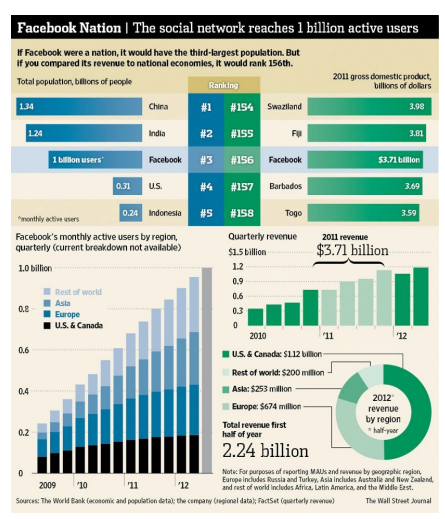
\includegraphics[width=\linewidth]{images/EsempioDV1.png} 
        \caption{Visualizzazione dati di Netflix}
        \label{fig:immagine1}
    \end{minipage}\hfill
    \begin{minipage}{0.45\textwidth}
        \centering
        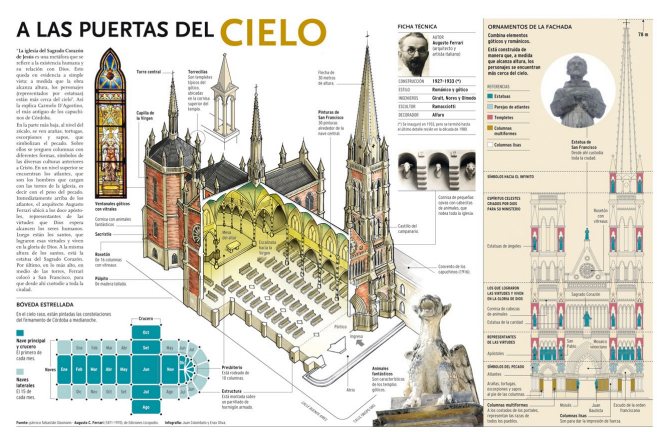
\includegraphics[width=\linewidth]{images/EsempioDV2.png} % Sostituisci 'immagine2' con il nome del tuo file immagine
        \caption{Juan Colombata \& Enzo Oliva  La Voz del Interior}
        \label{fig:immagine2}
    \end{minipage}
\end{figure}

Ci sono due prospettive diverse nell'interpretare l'Information Visualization:
\begin{itemize}
    \item  \textbf{Visualizzazione come scienza applicata:} Il valore di una buona visualizzazione consiste nel permetterci
     di individuare pattern nei dati e quindi la scienza della percezione dei pattern può fornire una 
     base per decisioni di design [C. Ware, Information Visualization. Perception for design, 2013].
    \item \textbf{Visualizzazione come tecnologia:}  Gli infografici sono uno strumento visivo per la comunicazione, la comprensione e l'analisi [A. Cairo, The functional art, 2013].
    Le limitazioni funzionali formano: come il design di un oggetto tecnologico deve dipendere dal compito che dovrebbe aiutare la forma grafica dovrebbe essere vincolata dalle funzioni della tua presentazione.
\end{itemize}
\subsubsection{Perchè la visualizzazione?}
Le visualizzazioni esplicative sono strumenti per presentare informazioni, comunicare dati e messaggi, 
spiegare qualcosa a qualcun altro, ha tre scopi principali: Explanation, confirmation e exploration.

Siamo una specie visiva. Il sistema visivo umano è molto bravo nell'identificare e analizzare i pattern.
Le visualizzazioni sono come artefatti cognitivi (strumenti che gli esseri umani hanno costruito per aiutare a pensare meglio, ad esempio l'abaco).
La visualizzazione ha a che fare con la cognizione distribuita (il nostro sistema cognitivo non è esclusivamente composto dal nostro cervello, 
mente e sensori, ma anche dall'ambiente intorno a noi, che utilizziamo per memorizzare e manipolare informazioni).
Le visualizzazioni permettono il trattamento parallelo delle informazioni, anziché sequenziale.
Le visualizzazioni esplorative sono strumenti per i lettori per analizzare ciò che
viene loro presentato. Molto spesso, l'esito dell'analisi esplorativa non è solo la risposta alle domande originali, ma la generazione di nuove domande.

\begin{figure}[H]
    \centering
    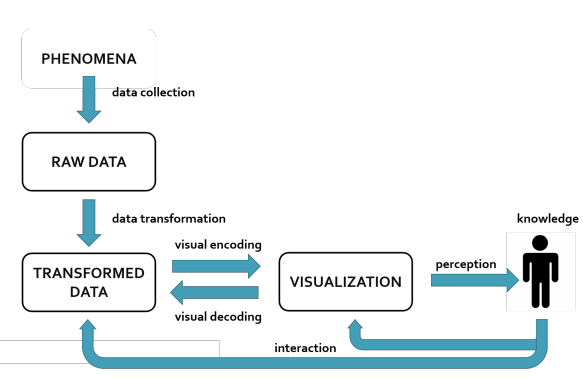
\includegraphics[width=0.5\textwidth]{images/visPipe.png} % Sostituisci 'nome_immagine' con il nome del tuo file immagine
    \caption{Visualization pipeline}
    \label{fig:immagine}
\end{figure}
\subsection{Fundamentals of 3D Computer Graphics}
Sono molti i campi dove si utilizza la \textbf{modellazione 3D}: 
Animazioni e serious gaming, 
Progettazione assistita da computer (CAD) e modellazione di prodotti, 
Patrimonio culturale, Archeologia, Architettura, Fabbricazione digitale e stampa 3D, Biologia e monitoraggio ambientale, 
Medicina e sistemi di eHealth, Moda del futuro, Sicurezza e difesa...
\\ Programma:
\begin{itemize}
\item  Modelli discreti per la rappresentazione dei dati in 3D (con un'attenzione particolare alle reti di triangoli) e tecniche di base di elaborazione 3D
\item Fondamenti della Grafica al Computer (tecniche di rendering, illuminazione e texture)
\item  Librerie e strumenti disponibili
\end{itemize}
\begin{figure}[H]
    \centering
    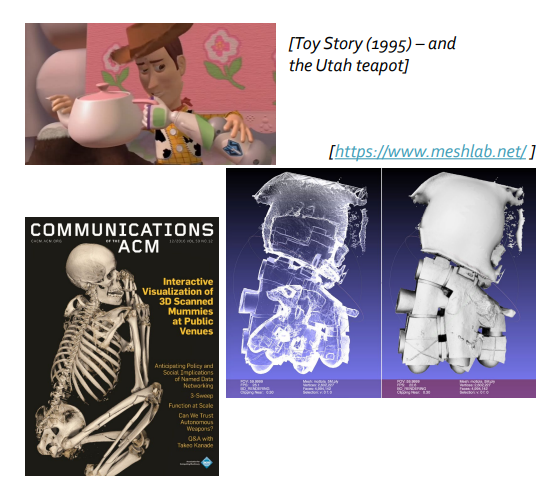
\includegraphics[width=0.5\textwidth]{images/3Dexp.png} % Sostituisci 'nome_immagine' con il nome del tuo file immagine
    \caption{Esempi di utlizzo dei modelli 3D}
    \label{fig:immagine}
\end{figure}
\subsection{Scientific Visualization}
Tecniche informatiche per la generazione di rappresentazioni visuali interattive di dati spazio-temporali acquisiti o simulati 
(collegamento naturale con il mondo 3D+tempo in cui viviamo). Le illustrazioni a la communicazione visuale della conoscienza è parte della nostra storia, anche oggi a causa dell'incremento 
della quantità dei dati da analizzare è necessario un approccio grafico per la visualizzaione.
La Visualizzazione Scientifica si applica in diversi campi come l'Ingegneria, la medicina e la Scienza.
La Visualizzazione Scientifica riguarda anche la definizione di algoritmi efficienti per la manipolazione interattiva ed esplorazione dei dati e delle loro caratteristiche.

\begin{figure}[H]
    \centering
    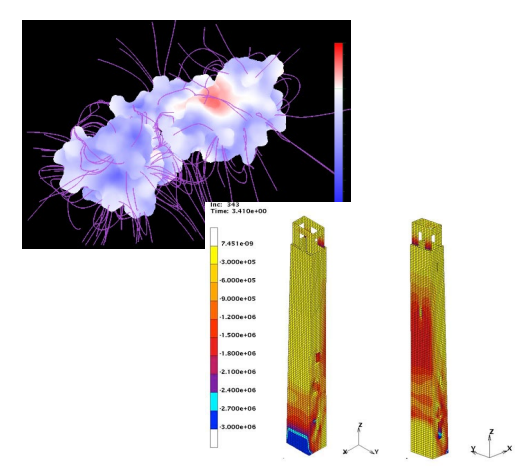
\includegraphics[width=0.5\textwidth]{images/ScientImage.png} % Sostituisci 'nome_immagine' con il nome del tuo file immagine
    \caption{Esempi di Visualizzazione Scientifica}
    \label{fig:immagine}
\end{figure}
